\providecommand{\val}[1]{\ifcsname num@#1\endcsname\csname num@#1\endcsname\else\textbf{??#1??}\fi}
\expandafter\def\csname num@BaseMultiDL\endcsname{-2.4}
\expandafter\def\csname num@BaseMultiDLci\endcsname{[-3.7, -0.9]}
\expandafter\def\csname num@BaseMultiDP\endcsname{+3.3}
\expandafter\def\csname num@BaseMultiDPci\endcsname{[+0.4, +6.1]}
\expandafter\def\csname num@BaseMultiFull\endcsname{221}
\expandafter\def\csname num@BaseMultiGreedy\endcsname{229}
\expandafter\def\csname num@BaseMultiLost\endcsname{13}
\expandafter\def\csname num@BaseMultiPairs\endcsname{240}
\expandafter\def\csname num@BaseMultiRescued\endcsname{5}
\expandafter\def\csname num@BaseSingleDL\endcsname{-0.9}
\expandafter\def\csname num@BaseSingleDLci\endcsname{[-1.8, -0.2]}
\expandafter\def\csname num@BaseSingleDP\endcsname{+1.1}
\expandafter\def\csname num@BaseSingleDPci\endcsname{[+0.0, +2.7]}
\expandafter\def\csname num@BaseSingleFull\endcsname{156}
\expandafter\def\csname num@BaseSingleGreedy\endcsname{158}
\expandafter\def\csname num@BaseSingleLost\endcsname{2}
\expandafter\def\csname num@BaseSinglePairs\endcsname{180}
\expandafter\def\csname num@BaseSingleRescued\endcsname{0}
\expandafter\def\csname num@Branch\endcsname{-0.3}
\expandafter\def\csname num@Branchci\endcsname{[-7.5, +6.9]}
\expandafter\def\csname num@BudgetDemoFour3D1024\endcsname{20/20}
\expandafter\def\csname num@BudgetDemoFour3D1024Depth\endcsname{2.9}
\expandafter\def\csname num@BudgetDemoFour3D1024Kept\endcsname{0.63}
\expandafter\def\csname num@BudgetDemoFour3D1024L\endcsname{12.8}
\expandafter\def\csname num@BudgetDemoFour3D16\endcsname{20/20}
\expandafter\def\csname num@BudgetDemoFour3D16Depth\endcsname{2.1}
\expandafter\def\csname num@BudgetDemoFour3D16Kept\endcsname{0.76}
\expandafter\def\csname num@BudgetDemoFour3D16L\endcsname{12.7}
\expandafter\def\csname num@BudgetDemoFour3D2000\endcsname{20/20}
\expandafter\def\csname num@BudgetDemoFour3D2000Depth\endcsname{3.0}
\expandafter\def\csname num@BudgetDemoFour3D2000Kept\endcsname{0.57}
\expandafter\def\csname num@BudgetDemoFour3D2000L\endcsname{12.4}
\expandafter\def\csname num@BudgetDemoFour3D256\endcsname{19/20}
\expandafter\def\csname num@BudgetDemoFour3D256Depth\endcsname{2.7}
\expandafter\def\csname num@BudgetDemoFour3D256Kept\endcsname{0.74}
\expandafter\def\csname num@BudgetDemoFour3D256L\endcsname{15.8}
\expandafter\def\csname num@BudgetDemoFour3D64\endcsname{20/20}
\expandafter\def\csname num@BudgetDemoFour3D64Depth\endcsname{2.5}
\expandafter\def\csname num@BudgetDemoFour3D64Kept\endcsname{0.77}
\expandafter\def\csname num@BudgetDemoFour3D64L\endcsname{12.5}
\expandafter\def\csname num@BudgetDemoOpen2D1024\endcsname{20/20}
\expandafter\def\csname num@BudgetDemoOpen2D1024Depth\endcsname{4.1}
\expandafter\def\csname num@BudgetDemoOpen2D1024Kept\endcsname{0.88}
\expandafter\def\csname num@BudgetDemoOpen2D1024L\endcsname{11.3}
\expandafter\def\csname num@BudgetDemoOpen2D16\endcsname{20/20}
\expandafter\def\csname num@BudgetDemoOpen2D16Depth\endcsname{2.5}
\expandafter\def\csname num@BudgetDemoOpen2D16Kept\endcsname{0.90}
\expandafter\def\csname num@BudgetDemoOpen2D16L\endcsname{11.4}
\expandafter\def\csname num@BudgetDemoOpen2D2000\endcsname{20/20}
\expandafter\def\csname num@BudgetDemoOpen2D2000Depth\endcsname{4.4}
\expandafter\def\csname num@BudgetDemoOpen2D2000Kept\endcsname{0.85}
\expandafter\def\csname num@BudgetDemoOpen2D2000L\endcsname{11.4}
\expandafter\def\csname num@BudgetDemoOpen2D256\endcsname{20/20}
\expandafter\def\csname num@BudgetDemoOpen2D256Depth\endcsname{3.5}
\expandafter\def\csname num@BudgetDemoOpen2D256Kept\endcsname{0.80}
\expandafter\def\csname num@BudgetDemoOpen2D256L\endcsname{11.4}
\expandafter\def\csname num@BudgetDemoOpen2D64\endcsname{20/20}
\expandafter\def\csname num@BudgetDemoOpen2D64Depth\endcsname{3.1}
\expandafter\def\csname num@BudgetDemoOpen2D64Kept\endcsname{0.77}
\expandafter\def\csname num@BudgetDemoOpen2D64L\endcsname{11.3}
\expandafter\def\csname num@BudgetFactorS10A26C51024\endcsname{19/20}
\expandafter\def\csname num@BudgetFactorS10A26C51024Depth\endcsname{3.1}
\expandafter\def\csname num@BudgetFactorS10A26C51024Kept\endcsname{0.65}
\expandafter\def\csname num@BudgetFactorS10A26C51024L\endcsname{15.4}
\expandafter\def\csname num@BudgetFactorS10A26C516\endcsname{18/20}
\expandafter\def\csname num@BudgetFactorS10A26C516Depth\endcsname{2.2}
\expandafter\def\csname num@BudgetFactorS10A26C516Kept\endcsname{0.82}
\expandafter\def\csname num@BudgetFactorS10A26C516L\endcsname{18.2}
\expandafter\def\csname num@BudgetFactorS10A26C52000\endcsname{19/20}
\expandafter\def\csname num@BudgetFactorS10A26C52000Depth\endcsname{3.2}
\expandafter\def\csname num@BudgetFactorS10A26C52000Kept\endcsname{0.61}
\expandafter\def\csname num@BudgetFactorS10A26C52000L\endcsname{16.0}
\expandafter\def\csname num@BudgetFactorS10A26C5256\endcsname{20/20}
\expandafter\def\csname num@BudgetFactorS10A26C5256Depth\endcsname{2.8}
\expandafter\def\csname num@BudgetFactorS10A26C5256Kept\endcsname{0.71}
\expandafter\def\csname num@BudgetFactorS10A26C5256L\endcsname{13.1}
\expandafter\def\csname num@BudgetFactorS10A26C564\endcsname{18/20}
\expandafter\def\csname num@BudgetFactorS10A26C564Depth\endcsname{2.6}
\expandafter\def\csname num@BudgetFactorS10A26C564Kept\endcsname{0.73}
\expandafter\def\csname num@BudgetFactorS10A26C564L\endcsname{17.8}
\expandafter\def\csname num@BudgetStrongWind1024\endcsname{20/20}
\expandafter\def\csname num@BudgetStrongWind1024Depth\endcsname{2.3}
\expandafter\def\csname num@BudgetStrongWind1024Kept\endcsname{0.71}
\expandafter\def\csname num@BudgetStrongWind1024L\endcsname{18.1}
\expandafter\def\csname num@BudgetStrongWind16\endcsname{20/20}
\expandafter\def\csname num@BudgetStrongWind16Depth\endcsname{1.7}
\expandafter\def\csname num@BudgetStrongWind16Kept\endcsname{0.84}
\expandafter\def\csname num@BudgetStrongWind16L\endcsname{16.2}
\expandafter\def\csname num@BudgetStrongWind2000\endcsname{18/20}
\expandafter\def\csname num@BudgetStrongWind2000Depth\endcsname{2.4}
\expandafter\def\csname num@BudgetStrongWind2000Kept\endcsname{0.76}
\expandafter\def\csname num@BudgetStrongWind2000L\endcsname{23.9}
\expandafter\def\csname num@BudgetStrongWind256\endcsname{19/20}
\expandafter\def\csname num@BudgetStrongWind256Depth\endcsname{2.0}
\expandafter\def\csname num@BudgetStrongWind256Kept\endcsname{0.78}
\expandafter\def\csname num@BudgetStrongWind256L\endcsname{21.0}
\expandafter\def\csname num@BudgetStrongWind64\endcsname{19/20}
\expandafter\def\csname num@BudgetStrongWind64Depth\endcsname{1.8}
\expandafter\def\csname num@BudgetStrongWind64Kept\endcsname{0.79}
\expandafter\def\csname num@BudgetStrongWind64L\endcsname{20.6}
\expandafter\def\csname num@CallsC0\endcsname{15,878}
\expandafter\def\csname num@CallsC5\endcsname{16,774}
\expandafter\def\csname num@CeilCorridor\endcsname{63.1}
\expandafter\def\csname num@CeilCorridorSim\endcsname{60.7}
\expandafter\def\csname num@CeilFourSingle\endcsname{94}
\expandafter\def\csname num@CeilFourUncoord\endcsname{16}
\expandafter\def\csname num@CeilFourUncoordCI\endcsname{[13.8, 18.3]\%}
\expandafter\def\csname num@CeilGap\endcsname{70.5}
\expandafter\def\csname num@CeilGapSim\endcsname{69.1}
\expandafter\def\csname num@ClutterNoisy\endcsname{+4.5}
\expandafter\def\csname num@ClutterNoisyA26\endcsname{+4.2}
\expandafter\def\csname num@ClutterNoisyA26ci\endcsname{[-0.6, +8.9]}
\expandafter\def\csname num@ClutterNoisyA6\endcsname{+4.8}
\expandafter\def\csname num@ClutterNoisyA6ci\endcsname{[+3.8, +5.7]}
\expandafter\def\csname num@ClutterNoisyci\endcsname{[+2.1, +6.8]}
\expandafter\def\csname num@ClutterQuiet\endcsname{+1.0}
\expandafter\def\csname num@ClutterQuietA26\endcsname{+0.2}
\expandafter\def\csname num@ClutterQuietA26ci\endcsname{[-0.1, +0.5]}
\expandafter\def\csname num@ClutterQuietA6\endcsname{+1.8}
\expandafter\def\csname num@ClutterQuietA6ci\endcsname{[+1.2, +2.3]}
\expandafter\def\csname num@ClutterQuietci\endcsname{[+0.7, +1.3]}
\expandafter\def\csname num@CompHeuristic\endcsname{+0.6}
\expandafter\def\csname num@CompHeuristicAhi\endcsname{+2.6}
\expandafter\def\csname num@CompHeuristicAint\endcsname{[+0.6, +7.3]}
\expandafter\def\csname num@CompHeuristicAlo\endcsname{-1.4}
\expandafter\def\csname num@CompHeuristicChi\endcsname{+1.7}
\expandafter\def\csname num@CompHeuristicCint\endcsname{[-1.4, +5.8]}
\expandafter\def\csname num@CompHeuristicClo\endcsname{-0.5}
\expandafter\def\csname num@CompHeuristicP\endcsname{-3.8}
\expandafter\def\csname num@CompHeuristicShi\endcsname{+0.6}
\expandafter\def\csname num@CompHeuristicSint\endcsname{[-2.7, +2.6]}
\expandafter\def\csname num@CompHeuristicSlo\endcsname{+0.6}
\expandafter\def\csname num@CompHeuristicci\endcsname{[-1.3, +2.5]}
\expandafter\def\csname num@CompMaxq\endcsname{+3.7}
\expandafter\def\csname num@CompMaxqAhi\endcsname{+1.0}
\expandafter\def\csname num@CompMaxqAint\endcsname{[-7.8, -3.2]}
\expandafter\def\csname num@CompMaxqAlo\endcsname{+6.5}
\expandafter\def\csname num@CompMaxqChi\endcsname{+6.8}
\expandafter\def\csname num@CompMaxqCint\endcsname{[+3.3, +8.9]}
\expandafter\def\csname num@CompMaxqClo\endcsname{+0.7}
\expandafter\def\csname num@CompMaxqP\endcsname{-3.8}
\expandafter\def\csname num@CompMaxqShi\endcsname{+2.6}
\expandafter\def\csname num@CompMaxqSint\endcsname{[-4.7, +0.3]}
\expandafter\def\csname num@CompMaxqSlo\endcsname{+4.8}
\expandafter\def\csname num@CompMaxqci\endcsname{[+2.4, +5.1]}
\expandafter\def\csname num@CompNoguidance\endcsname{+35.7}
\expandafter\def\csname num@CompNoguidanceAhi\endcsname{+37.5}
\expandafter\def\csname num@CompNoguidanceAint\endcsname{[-2.0, +9.0]}
\expandafter\def\csname num@CompNoguidanceAlo\endcsname{+34.0}
\expandafter\def\csname num@CompNoguidanceChi\endcsname{+42.3}
\expandafter\def\csname num@CompNoguidanceCint\endcsname{[+8.7, +17.5]}
\expandafter\def\csname num@CompNoguidanceClo\endcsname{+29.1}
\expandafter\def\csname num@CompNoguidanceP\endcsname{-50.0}
\expandafter\def\csname num@CompNoguidanceShi\endcsname{+33.8}
\expandafter\def\csname num@CompNoguidanceSint\endcsname{[-8.1, +0.2]}
\expandafter\def\csname num@CompNoguidanceSlo\endcsname{+37.7}
\expandafter\def\csname num@CompNoguidanceci\endcsname{[+33.6, +37.8]}
\expandafter\def\csname num@CompNoleaf\endcsname{+0.5}
\expandafter\def\csname num@CompNoleafAhi\endcsname{+0.9}
\expandafter\def\csname num@CompNoleafAint\endcsname{[-1.5, +3.1]}
\expandafter\def\csname num@CompNoleafAlo\endcsname{+0.1}
\expandafter\def\csname num@CompNoleafChi\endcsname{+1.3}
\expandafter\def\csname num@CompNoleafCint\endcsname{[-1.2, +4.4]}
\expandafter\def\csname num@CompNoleafClo\endcsname{-0.3}
\expandafter\def\csname num@CompNoleafP\endcsname{-1.9}
\expandafter\def\csname num@CompNoleafShi\endcsname{+0.3}
\expandafter\def\csname num@CompNoleafSint\endcsname{[-2.5, +1.6]}
\expandafter\def\csname num@CompNoleafSlo\endcsname{+0.7}
\expandafter\def\csname num@CompNoleafci\endcsname{[-1.0, +2.0]}
\expandafter\def\csname num@CompNorisk\endcsname{+1.8}
\expandafter\def\csname num@CompNoriskAhi\endcsname{+2.3}
\expandafter\def\csname num@CompNoriskAint\endcsname{[-2.1, +4.0]}
\expandafter\def\csname num@CompNoriskAlo\endcsname{+1.3}
\expandafter\def\csname num@CompNoriskChi\endcsname{+3.7}
\expandafter\def\csname num@CompNoriskCint\endcsname{[+0.4, +7.0]}
\expandafter\def\csname num@CompNoriskClo\endcsname{-0.1}
\expandafter\def\csname num@CompNoriskP\endcsname{-4.4}
\expandafter\def\csname num@CompNoriskShi\endcsname{+1.5}
\expandafter\def\csname num@CompNoriskSint\endcsname{[-3.9, +2.6]}
\expandafter\def\csname num@CompNoriskSlo\endcsname{+2.1}
\expandafter\def\csname num@CompNoriskci\endcsname{[+0.1, +3.5]}
\expandafter\def\csname num@CompNowidening\endcsname{+1.0}
\expandafter\def\csname num@CompNowideningAhi\endcsname{+2.4}
\expandafter\def\csname num@CompNowideningAint\endcsname{[-0.2, +5.6]}
\expandafter\def\csname num@CompNowideningAlo\endcsname{-0.3}
\expandafter\def\csname num@CompNowideningChi\endcsname{+2.1}
\expandafter\def\csname num@CompNowideningCint\endcsname{[-0.8, +5.3]}
\expandafter\def\csname num@CompNowideningClo\endcsname{-0.1}
\expandafter\def\csname num@CompNowideningP\endcsname{-2.5}
\expandafter\def\csname num@CompNowideningShi\endcsname{+0.9}
\expandafter\def\csname num@CompNowideningSint\endcsname{[-3.2, +2.8]}
\expandafter\def\csname num@CompNowideningSlo\endcsname{+1.1}
\expandafter\def\csname num@CompNowideningci\endcsname{[-0.5, +2.5]}
\expandafter\def\csname num@CompVisitschoice\endcsname{+3.2}
\expandafter\def\csname num@CompVisitschoiceAhi\endcsname{+0.7}
\expandafter\def\csname num@CompVisitschoiceAint\endcsname{[-7.1, -3.0]}
\expandafter\def\csname num@CompVisitschoiceAlo\endcsname{+5.7}
\expandafter\def\csname num@CompVisitschoiceChi\endcsname{+5.7}
\expandafter\def\csname num@CompVisitschoiceCint\endcsname{[+2.8, +7.4]}
\expandafter\def\csname num@CompVisitschoiceClo\endcsname{+0.7}
\expandafter\def\csname num@CompVisitschoiceP\endcsname{-1.2}
\expandafter\def\csname num@CompVisitschoiceShi\endcsname{+2.6}
\expandafter\def\csname num@CompVisitschoiceSint\endcsname{[-3.3, +0.9]}
\expandafter\def\csname num@CompVisitschoiceSlo\endcsname{+3.8}
\expandafter\def\csname num@CompVisitschoiceci\endcsname{[+2.1, +4.3]}
\expandafter\def\csname num@DemoCapShare\endcsname{99}
\expandafter\def\csname num@DemoCapped\endcsname{73}
\expandafter\def\csname num@DemoDecisions\endcsname{74}
\expandafter\def\csname num@DemoMaxPlan\endcsname{9.21}
\expandafter\def\csname num@DemoMinSims\endcsname{1,815}
\expandafter\def\csname num@DepthAlpha005\endcsname{3.5}
\expandafter\def\csname num@DepthAlpha20\endcsname{2.0}
\expandafter\def\csname num@DepthN1\endcsname{3.1}
\expandafter\def\csname num@DepthN4\endcsname{2.5}
\expandafter\def\csname num@DevEpisodes\endcsname{2,880}
\expandafter\def\csname num@DevSettings\endcsname{18}
\expandafter\def\csname num@EffAL\endcsname{-3.8}
\expandafter\def\csname num@EffALci\endcsname{[-5.8, -1.9]}
\expandafter\def\csname num@EffAP\endcsname{-1.1}
\expandafter\def\csname num@EffAPci\endcsname{[-5.2, +3.0]}
\expandafter\def\csname num@EffCL\endcsname{+3.7}
\expandafter\def\csname num@EffCLci\endcsname{[+2.5, +4.9]}
\expandafter\def\csname num@EffCP\endcsname{-2.2}
\expandafter\def\csname num@EffCPci\endcsname{[-4.9, +0.5]}
\expandafter\def\csname num@EffSL\endcsname{+0.5}
\expandafter\def\csname num@EffSLci\endcsname{[-0.9, +1.9]}
\expandafter\def\csname num@EffSP\endcsname{-1.1}
\expandafter\def\csname num@EffSPci\endcsname{[-4.0, +1.8]}
\expandafter\def\csname num@FactCollisions\endcsname{13}
\expandafter\def\csname num@FactObstacle\endcsname{12}
\expandafter\def\csname num@FactSuccess\endcsname{97.6}
\expandafter\def\csname num@FactTimeouts\endcsname{0}
\expandafter\def\csname num@FactVehicle\endcsname{1}
\expandafter\def\csname num@GuideA\endcsname{1539}
\expandafter\def\csname num@GuideB\endcsname{1540}
\expandafter\def\csname num@GuideDL\endcsname{-0.8}
\expandafter\def\csname num@GuideDLci\endcsname{[-1.4, -0.3]}
\expandafter\def\csname num@GuideDP\endcsname{+0.1}
\expandafter\def\csname num@GuideDPci\endcsname{[-0.9, +1.1]}
\expandafter\def\csname num@GuideDuplicates\endcsname{80}
\expandafter\def\csname num@GuideLosses\endcsname{43}
\expandafter\def\csname num@GuidePairs\endcsname{1,680}
\expandafter\def\csname num@GuideWins\endcsname{44}
\expandafter\def\csname num@IntAC\endcsname{-3.6}
\expandafter\def\csname num@IntACci\endcsname{[-4.5, -2.7]}
\expandafter\def\csname num@IntSA\endcsname{-5.0}
\expandafter\def\csname num@IntSAci\endcsname{[-8.3, -1.7]}
\expandafter\def\csname num@IntSC\endcsname{+0.7}
\expandafter\def\csname num@IntSCci\endcsname{[-2.0, +3.5]}
\expandafter\def\csname num@PairAS\endcsname{-4.3}
\expandafter\def\csname num@PairASci\endcsname{[-7.4, -1.3]}
\expandafter\def\csname num@PairCA\endcsname{+7.6}
\expandafter\def\csname num@PairCAci\endcsname{[+5.3, +9.8]}
\expandafter\def\csname num@PairCS\endcsname{+3.2}
\expandafter\def\csname num@PairCSci\endcsname{[+1.7, +4.7]}
\expandafter\def\csname num@ProbeBase\endcsname{69/80}
\expandafter\def\csname num@ProbeBaseGapSteps\endcsname{26}
\expandafter\def\csname num@ProbeRisk\endcsname{65/80}
\expandafter\def\csname num@ProbeRiskGapSteps\endcsname{19}
\expandafter\def\csname num@RandAlpha005\endcsname{40/40}
\expandafter\def\csname num@RandAlpha025\endcsname{38/40}
\expandafter\def\csname num@RandAlpha10\endcsname{36/40}
\expandafter\def\csname num@RandAlpha20\endcsname{30/40}
\expandafter\def\csname num@RandLowNoise\endcsname{78/80}
\expandafter\def\csname num@RandN1\endcsname{38/40}
\expandafter\def\csname num@RandN2\endcsname{36/40}
\expandafter\def\csname num@RandN3\endcsname{38/40}
\expandafter\def\csname num@RandN4\endcsname{32/40}
\expandafter\def\csname num@RandNFourHigh\endcsname{6/10}
\expandafter\def\csname num@RandNFourLow\endcsname{20/20}
\expandafter\def\csname num@RandObstacle\endcsname{9}
\expandafter\def\csname num@RandOverall\endcsname{144/160}
\expandafter\def\csname num@RandTimeouts\endcsname{0}
\expandafter\def\csname num@RandVehicle\endcsname{7}
\expandafter\def\csname num@RegAltitudeDetour\endcsname{20/20}
\expandafter\def\csname num@RegDemoFour3D\endcsname{20/20}
\expandafter\def\csname num@RegDemoOpen2D\endcsname{20/20}
\expandafter\def\csname num@RegNarrowPassage\endcsname{15/20}
\expandafter\def\csname num@RegStrongWind\endcsname{18/20}
\expandafter\def\csname num@RootA26\endcsname{22.4}
\expandafter\def\csname num@RootA6\endcsname{19.1}
\expandafter\def\csname num@RootC0\endcsname{21.8}
\expandafter\def\csname num@RootC5\endcsname{20.7}
\expandafter\def\csname num@SameSTen\endcsname{102}
\expandafter\def\csname num@SameSTotal\endcsname{180}
\expandafter\def\csname num@SetupS20\endcsname{381}
\expandafter\def\csname num@SetupS5\endcsname{95}
\expandafter\def\csname num@SuppFull\endcsname{127/140}
\expandafter\def\csname num@SuppGapRoute\endcsname{11}
\expandafter\def\csname num@SuppGapSteps\endcsname{20}
\expandafter\def\csname num@SuppGapStepsA\endcsname{39}
\expandafter\def\csname num@SuppGreedy\endcsname{125/140}
\expandafter\def\csname num@SuppSuppLayersCross2D\endcsname{20/20}
\expandafter\def\csname num@SuppSuppLayersFour2D\endcsname{20/20}
\expandafter\def\csname num@SuppSuppSingleClutter2D\endcsname{20/20}
\expandafter\def\csname num@SuppSuppSingleExample2D\endcsname{20/20}
\expandafter\def\csname num@SuppSuppSingleSlalom2D\endcsname{20/20}
\expandafter\def\csname num@SuppSuppSingleWallgap2D\endcsname{14/20}
\expandafter\def\csname num@SuppSuppYieldCorridor\endcsname{13/20}
\expandafter\def\csname num@SuppTimeouts\endcsname{0}
\expandafter\def\csname num@TopA26\endcsname{5.8}
\expandafter\def\csname num@TopA6\endcsname{10.7}
\expandafter\def\csname num@TopN1\endcsname{9.0}
\expandafter\def\csname num@TopN4\endcsname{7.2}
\expandafter\def\csname num@TotalEpisodes\endcsname{3,460}
\expandafter\def\csname num@TuneAnchorZ1\endcsname{133/160}
\expandafter\def\csname num@TuneAnchorZ1Eps0\endcsname{133/160}
\expandafter\def\csname num@TuneAnchorZ1W05\endcsname{140/160}
\expandafter\def\csname num@TuneAnchorZ2\endcsname{136/160}
\expandafter\def\csname num@TuneDijkstra\endcsname{140/160}
\expandafter\def\csname num@TuneDijkstraMaxq\endcsname{130/160}
\expandafter\def\csname num@TuneGreedyDijkstra\endcsname{138/160}
\expandafter\def\csname num@TuneGreedyRisk0\endcsname{121/160}
\expandafter\def\csname num@TuneGreedyRisk1\endcsname{138/160}
\expandafter\def\csname num@TuneGreedyVi\endcsname{142/160}
\expandafter\def\csname num@TuneRisk0\endcsname{125/160}
\expandafter\def\csname num@TuneRisk03\endcsname{130/160}
\expandafter\def\csname num@TuneRisk1\endcsname{129/160}
\expandafter\def\csname num@TuneRisk1C01\endcsname{129/160}
\expandafter\def\csname num@TuneRisk1C1\endcsname{123/160}
\expandafter\def\csname num@TuneRisk3\endcsname{126/160}
\expandafter\def\csname num@TuneVi\endcsname{143/160}
\expandafter\def\csname num@TuneViMaxq\endcsname{137/160}

\newcommand{\FactorialRows}{%
5 & 36 & 0 & 20/20 & 13.3 $\pm$ 0.9 & 134.1 $\pm$ 3.9 & 18,413 \\
5 & 36 & 2 & 19/20 & 21.8 $\pm$ 4.6 & 99.0 $\pm$ 23.0 & 19,010 \\
5 & 36 & 5 & 18/20 & 23.4 $\pm$ 6.1 & 89.1 $\pm$ 30.9 & 18,539 \\
5 & 324 & 0 & 20/20 & 12.1 $\pm$ 0.6 & 140.0 $\pm$ 2.1 & 14,951 \\
5 & 324 & 2 & 19/20 & 15.8 $\pm$ 4.9 & 117.8 $\pm$ 35.1 & 16,166 \\
5 & 324 & 5 & 18/20 & 18.1 $\pm$ 6.7 & 110.7 $\pm$ 34.1 & 15,664 \\
5 & 676 & 0 & 20/20 & 12.1 $\pm$ 0.7 & 140.0 $\pm$ 2.2 & 14,730 \\
5 & 676 & 2 & 20/20 & 13.2 $\pm$ 0.9 & 135.7 $\pm$ 3.1 & 15,330 \\
5 & 676 & 5 & 19/20 & 16.2 $\pm$ 4.9 & 120.7 $\pm$ 24.7 & 15,284 \\
10 & 36 & 0 & 20/20 & 13.8 $\pm$ 0.7 & 133.0 $\pm$ 2.5 & 18,368 \\
10 & 36 & 2 & 20/20 & 17.9 $\pm$ 1.2 & 116.0 $\pm$ 4.6 & 18,599 \\
10 & 36 & 5 & 19/20 & 28.1 $\pm$ 3.9 & 75.5 $\pm$ 28.1 & 19,998 \\
10 & 324 & 0 & 20/20 & 12.1 $\pm$ 0.6 & 139.8 $\pm$ 2.0 & 14,939 \\
10 & 324 & 2 & 20/20 & 13.2 $\pm$ 0.7 & 135.7 $\pm$ 2.5 & 15,738 \\
10 & 324 & 5 & 20/20 & 15.7 $\pm$ 0.8 & 125.4 $\pm$ 3.1 & 17,113 \\
10 & 676 & 0 & 20/20 & 12.2 $\pm$ 0.6 & 139.5 $\pm$ 2.1 & 14,759 \\
10 & 676 & 2 & 20/20 & 13.0 $\pm$ 0.7 & 136.7 $\pm$ 2.3 & 15,264 \\
10 & 676 & 5 & 19/20 & 16.8 $\pm$ 4.8 & 115.2 $\pm$ 33.6 & 16,457 \\
20 & 36 & 0 & 20/20 & 13.8 $\pm$ 0.7 & 133.0 $\pm$ 2.5 & 18,368 \\
20 & 36 & 2 & 19/20 & 20.0 $\pm$ 4.6 & 104.8 $\pm$ 23.2 & 18,891 \\
20 & 36 & 5 & 20/20 & 25.4 $\pm$ 1.4 & 90.0 $\pm$ 3.5 & 19,787 \\
20 & 324 & 0 & 20/20 & 12.1 $\pm$ 0.6 & 139.8 $\pm$ 2.0 & 14,939 \\
20 & 324 & 2 & 20/20 & 13.1 $\pm$ 0.7 & 135.6 $\pm$ 2.9 & 15,738 \\
20 & 324 & 5 & 19/20 & 17.8 $\pm$ 4.7 & 114.5 $\pm$ 24.0 & 17,184 \\
20 & 676 & 0 & 20/20 & 12.2 $\pm$ 0.6 & 139.5 $\pm$ 2.1 & 14,759 \\
20 & 676 & 2 & 19/20 & 15.4 $\pm$ 5.0 & 119.6 $\pm$ 35.3 & 15,672 \\
20 & 676 & 5 & 19/20 & 16.4 $\pm$ 4.9 & 120.1 $\pm$ 24.6 & 16,513 \\
}

\newcommand{\FactorEffectRows}{%
State size & -2.0 & [-4.4, 0.3] \\
Action size & -10.2 & [-12.5, -8.0] \\
Clutter & 9.5 & [6.4, 12.5] \\
}

\newcommand{\ComponentRows}{%
Uniform proposals/rollouts & +34.4 [+31.5, +37.4] & -50.0 [-56.0, -44.0] & +33.5 / +35.3 & +34.0 / +34.9 & +30.6 / +38.2$^\ast$ \\
Zero leaf value & +0.0 [-1.5, +1.5] & +0.6 [-2.4, +3.6] & -1.2 / +1.2 & -0.1 / +0.1 & -0.1 / +0.2 \\
No progressive widening & +0.1 [-1.4, +1.5] & +0.0 [-3.3, +3.3] & +0.0 / +0.1 & -0.5 / +0.7 & +0.2 / -0.0 \\
Risk-free guidance & -0.1 [-1.4, +1.2] & -1.9 [-4.7, +1.0] & +0.9 / -1.1 & +0.1 / -0.3 & +0.1 / -0.3 \\
Most-visited final action & +3.4 [+1.7, +5.0] & -1.9 [-6.2, +2.5] & +3.7 / +3.0 & +5.2 / +1.6$^\ast$ & +0.4 / +6.3$^\ast$ \\
Guided policy, no search & -0.4 [-1.7, +0.9] & -0.6 [-3.6, +2.4] & -0.6 / -0.3 & -0.9 / +0.1 & -0.1 / -0.7 \\
}

\newcommand{\ComponentRawRows}{%
Full solver & 20/20 & 18/20 & 20/20 & 19/20 & 20/20 & 20/20 & 20/20 & 19/20 \\
Uniform proposals/rollouts & 9/10 & 0/10 & 9/10 & 0/10 & 10/10 & 0/10 & 9/10 & 0/10 \\
Zero leaf value & 20/20 & 20/20 & 20/20 & 18/20 & 20/20 & 20/20 & 20/20 & 19/20 \\
No progressive widening & 20/20 & 19/20 & 20/20 & 18/20 & 20/20 & 20/20 & 20/20 & 19/20 \\
Risk-free guidance & 20/20 & 16/20 & 20/20 & 19/20 & 20/20 & 19/20 & 20/20 & 19/20 \\
Most-visited final action & 20/20 & 19/20 & 20/20 & 18/20 & 20/20 & 19/20 & 20/20 & 17/20 \\
Guided policy, no search & 20/20 & 18/20 & 20/20 & 19/20 & 20/20 & 19/20 & 20/20 & 19/20 \\
}

\newcommand{\BudgetRows}{%
Open 2D (1) & 16 & 20/20 & 11.4 $\pm$ 0.4 & 2.0 & 2.48 \\
Open 2D (1) & 64 & 20/20 & 11.4 $\pm$ 0.4 & 4.0 & 3.07 \\
Open 2D (1) & 256 & 20/20 & 11.4 $\pm$ 0.4 & 7.7 & 3.54 \\
Open 2D (1) & 1,024 & 20/20 & 11.4 $\pm$ 0.4 & 7.7 & 4.10 \\
Open 2D (1) & 2,000 & 20/20 & 11.3 $\pm$ 0.3 & 7.7 & 4.41 \\
Strong wind (1) & 16 & 19/20 & 21.1 $\pm$ 6.8 & 2.0 & 1.53 \\
Strong wind (1) & 64 & 17/20 & 27.9 $\pm$ 10.8 & 4.0 & 1.72 \\
Strong wind (1) & 256 & 18/20 & 25.4 $\pm$ 9.0 & 8.0 & 1.95 \\
Strong wind (1) & 1,024 & 18/20 & 28.0 $\pm$ 8.9 & 15.0 & 2.20 \\
Strong wind (1) & 2,000 & 18/20 & 26.3 $\pm$ 8.9 & 17.3 & 2.35 \\
Four 3D (4) & 16 & 20/20 & 13.1 $\pm$ 0.7 & 2.0 & 1.95 \\
Four 3D (4) & 64 & 19/20 & 16.2 $\pm$ 7.1 & 4.0 & 2.29 \\
Four 3D (4) & 256 & 20/20 & 12.8 $\pm$ 0.7 & 8.0 & 2.48 \\
Four 3D (4) & 1,024 & 20/20 & 12.9 $\pm$ 0.6 & 16.0 & 2.67 \\
Four 3D (4) & 2,000 & 20/20 & 12.8 $\pm$ 0.6 & 22.8 & 2.75 \\
Factorial S10/A26/C5 (2) & 16 & 19/20 & 17.1 $\pm$ 4.8 & 2.0 & 2.10 \\
Factorial S10/A26/C5 (2) & 64 & 18/20 & 19.2 $\pm$ 6.6 & 4.0 & 2.54 \\
Factorial S10/A26/C5 (2) & 256 & 18/20 & 19.4 $\pm$ 6.6 & 8.0 & 2.79 \\
Factorial S10/A26/C5 (2) & 1,024 & 18/20 & 19.1 $\pm$ 6.6 & 15.9 & 3.03 \\
Factorial S10/A26/C5 (2) & 2,000 & 19/20 & 16.8 $\pm$ 4.8 & 22.5 & 3.13 \\
}

\newcommand{\ClutterControlRows}{%
all 26 & 0.25 & 0 & 20/20 & 12.2 $\pm$ 0.6 & 0 & 0 \\
 &  & 2 & 20/20 & 13.0 $\pm$ 0.7 & 0 & 0 \\
 &  & 5 & 19/20 & 16.8 $\pm$ 4.8 & 0 & 1 \\
 & 0.01 & 0 & 20/20 & 11.0 $\pm$ 0.0 & 0 & 0 \\
 &  & 2 & 20/20 & 11.0 $\pm$ 0.0 & 0 & 0 \\
 &  & 5 & 20/20 & 11.2 $\pm$ 0.2 & 0 & 0 \\
axial 6 & 0.25 & 0 & 20/20 & 13.8 $\pm$ 0.7 & 0 & 0 \\
 &  & 2 & 20/20 & 17.9 $\pm$ 1.2 & 0 & 0 \\
 &  & 5 & 19/20 & 28.1 $\pm$ 3.9 & 0 & 1 \\
 & 0.01 & 0 & 20/20 & 11.6 $\pm$ 0.4 & 0 & 0 \\
 &  & 2 & 20/20 & 13.2 $\pm$ 0.3 & 0 & 0 \\
 &  & 5 & 20/20 & 14.4 $\pm$ 0.5 & 0 & 0 \\
}

\newcommand{\BranchControlRows}{%
$\times1$ & 676 & 19/20 & 14.9 $\pm$ 5.0 & 22.3 & 5.7 \\
$\times2$ & 2,704 & 19/20 & 14.7 $\pm$ 5.0 & 23.0 & 5.1 \\
$\times4$ & 10,816 & 19/20 & 14.6 $\pm$ 5.0 & 23.0 & 5.0 \\
}

\newcommand{\RandomRows}{%
Drones $N$ & 1 & 38/40 & [83, 99] & 10.8 $\pm$ 3.7 & 3.15 \\
 & 2 & 36/40 & [77, 96] & 15.6 $\pm$ 5.0 & 2.77 \\
 & 3 & 38/40 & [83, 99] & 14.2 $\pm$ 3.7 & 2.54 \\
 & 4 & 32/40 & [65, 90] & 21.2 $\pm$ 6.5 & 2.48 \\
Noise $\alpha$ & 0.05 & 40/40 & [91, 100] & 7.7 $\pm$ 0.3 & 3.51 \\
 & 0.25 & 38/40 & [83, 99] & 11.0 $\pm$ 3.7 & 3.10 \\
 & 1 & 36/40 & [77, 96] & 16.0 $\pm$ 4.8 & 2.31 \\
 & 2 & 30/40 & [60, 86] & 27.1 $\pm$ 6.4 & 2.02 \\
}

\newcommand{\RegressionRows}{%
\texttt{demo\_open\_2d} & 20/20 & 0 & 11.7 $\pm$ 0.5 & 0.0380 \\
\texttt{demo\_four\_3d} & 19/20 & 1 & 16.3 $\pm$ 7.0 & 0.0378 \\
\texttt{already\_at\_goals} & 20/20 & 0 & 0.0 $\pm$ 0.0 & 0.0000 \\
\texttt{single\_cell\_goal} & 20/20 & 0 & 0.0 $\pm$ 0.0 & 0.0000 \\
\texttt{one\_reached} & 20/20 & 0 & 8.6 $\pm$ 0.5 & 0.0437 \\
\texttt{swap\_2d} & 20/20 & 0 & 5.2 $\pm$ 0.3 & 0.0379 \\
\texttt{boundary\_reverse} & 20/20 & 0 & 6.0 $\pm$ 0.5 & 0.0377 \\
\texttt{tiny\_2d} & 20/20 & 0 & 1.1 $\pm$ 0.1 & 0.0375 \\
\texttt{thin\_1d} & 20/20 & 0 & 9.8 $\pm$ 1.4 & 0.0374 \\
\texttt{infeasible\_altitude} & 0/20 & 0 & 80.0 $\pm$ 0.0 & 0.0000 \\
\texttt{infeasible\_wall} & 0/20 & 0 & 80.0 $\pm$ 0.0 & 0.0000 \\
\texttt{infeasible\_shared\_goal} & 0/20 & 0 & 80.0 $\pm$ 0.0 & 0.0000 \\
\texttt{horizon\_one} & 0/20 & 0 & 1.0 $\pm$ 0.0 & 0.0489 \\
\texttt{narrow\_passage} & 16/20 & 4 & 27.5 $\pm$ 12.7 & 0.0383 \\
\texttt{altitude\_detour} & 17/20 & 3 & 20.6 $\pm$ 12.0 & 0.0478 \\
\texttt{strong\_wind} & 14/20 & 6 & 39.5 $\pm$ 13.0 & 0.0376 \\
\texttt{three\_3d} & 18/20 & 2 & 17.4 $\pm$ 10.0 & 0.0525 \\
\texttt{four\_2d} & 16/20 & 4 & 24.3 $\pm$ 13.4 & 0.0383 \\
}

\newcommand{\TuningRows}{%
1 & risk0 & 125/160 & 20 & 15 & 24.3 $\pm$ 3.1 & -9.4 [-15.4, -3.3] & +4.5 [+2.1, +7.0] \\
1 & risk0.3 & 130/160 & 19 & 8 & 23.4 $\pm$ 2.9 & -6.2 [-12.2, -0.3] & +3.7 [+1.2, +6.1] \\
1 & risk1 & 129/160 & 20 & 9 & 23.4 $\pm$ 3.0 & -6.9 [-13.4, -0.4] & +3.7 [+0.6, +6.8] \\
1 & risk3 & 126/160 & 23 & 7 & 23.8 $\pm$ 3.0 & -8.8 [-15.5, -2.0] & +4.1 [+1.2, +7.0] \\
1 & risk1\_c0.1 & 129/160 & 21 & 8 & 23.0 $\pm$ 2.9 & -6.9 [-12.2, -1.5] & +3.3 [+1.4, +5.2] \\
1 & risk1\_c1 & 123/160 & 28 & 8 & 25.1 $\pm$ 3.2 & -10.6 [-15.4, -5.9] & +5.4 [+3.3, +7.5] \\
1 & greedy\_risk0 & 121/160 & 17 & 22 & 23.9 $\pm$ 3.2 & -11.9 [-15.8, -8.0] & +4.2 [+2.0, +6.4] \\
1 & greedy\_risk1 & 138/160 & 19 & 4 & 19.8 $\pm$ 2.6 & -1.2 [-5.4, +2.9] & +0.1 [-1.5, +1.6] \\
2 & anchor\_z1 & 133/160 & 19 & 8 & 21.3 $\pm$ 2.8 & -4.4 [-8.6, -0.1] & +1.6 [-0.1, +3.3] \\
2 & anchor\_z2 & 136/160 & 18 & 6 & 20.7 $\pm$ 2.7 & -2.5 [-7.3, +2.3] & +0.9 [-0.6, +2.4] \\
2 & anchor\_z1\_eps0 & 133/160 & 21 & 6 & 21.4 $\pm$ 2.8 & -4.4 [-7.4, -1.4] & +1.7 [+0.6, +2.8] \\
2 & anchor\_z1\_w0.5 & 140/160 & 13 & 9 & 19.7 $\pm$ 2.5 & --- & --- \\
}

\section*{Part B: Multi-drone planning under uncertainty (35 points)}
\begingroup
\setlength{\parindent}{0pt}
\setlength{\parskip}{4pt}

\subsection*{Question 1: MDP formulation (3 points)}
Let $\mathcal G=\{0,\ldots,n_x-1\}\times\{0,\ldots,n_y-1\}
\times\{0,\ldots,n_z-1\}$, with obstacles $O$ and known drone goals $g_i$.
The finite-horizon MDP is $(\mathcal S,\mathcal A,T,R,\gamma)$.

\textbf{States and actions.} A live state is
\[
 s=\bigl((p_i,r_i)_{i=1}^{N},t\bigr),\qquad 0\le t<H,
\]
where $p_i$ is drone $i$'s cell and $r_i$ indicates that it has reached its
goal. Reached drones remain at their goals and occupy those cells.
The state space also contains an absorbing state $\bot$, entered after a
collision, all goals being reached, or the step limit $H$.
Each active drone commands one of $B=26$ neighbour offsets (or $B=8$ with
fixed altitude), giving $\mathcal A=\{0,\ldots,B-1\}^{N}$.
There is no hover action; reached drones ignore their commands.

\textbf{Transitions.} Let $q_i(y_i\mid p_i,r_i,a_i)$ be the supplied,
normalised single-drone target law (Appendix~\ref{app:guidance}).
For a reached drone, $q_i(y_i\mid p_i,1,a_i)=\mathbf1\{y_i=p_i\}$.
Raw targets $y=(y_1,\ldots,y_N)$ are conditionally independent.
Let $F(s,y)$ apply the simulator's position and flag updates and return
$\bot$ on termination. Then
\[
 T(s,a,s')=\sum_{y:F(s,y)=s'}\prod_{i=1}^{N}
 q_i(y_i\mid p_i,r_i,a_i),\qquad T(\bot,a,\bot)=1.
\]
An obstacle hit or shared returned cell terminates the mission; cell swaps
and diagonal crossings are permitted by the supplied collision rule.

\textbf{Reward and objective.} For a sampled outcome $y$, let $K_O$ count
obstacle hits, $K_V$ count drones in shared-cell groups, and $\Delta r_i$
indicate a newly reached goal. The simulator returns
\[
 \widetilde r(s,a,y)=Nc_{\mathrm{step}}+C(K_O+K_V)+G\sum_i\Delta r_i,
 \qquad c_{\mathrm{step}}<0,\ C<0,\ G>0.
\]
Thus $R(s,a)=\mathbb E_y[\widetilde r(s,a,y)\mid s,a]$ and $R(\bot,a)=0$.
The terminal transition receives its reward before absorption. The objective is
\[
 \max_\mu\ \mathbb E_\mu\!\left[
 \sum_{t=0}^{\tau-1}\gamma^t\widetilde r_t\right],
 \qquad \tau=\min\{T_{\mathrm{success}},T_{\mathrm{collision}},H\}.
\]
This encourages fast completion and penalises collisions.

\subsection*{Question 2: Approximate online solver (4 points)}
I use UCT/MCTS with progressive widening~\cite{mdp-lectures,kocsis2006,couetoux2011},
re-planned after every executed step. The supplied generative model samples
outcomes without enumerating the state space or all $26^4=456{,}976$ joint
actions.

\textbf{Guidance.} Cached Dijkstra maps $J_i$ trade path length against
one-step obstacle-slip risk. For a command from $p_i$ towards $q$, the score is
\[
 J_i(q)+0.025\|q-g_i\|_1+\frac{0.3}{\max\{1,d(q)\}}
 +\lambda\ell(p_i)\sum_{\substack{k\ne i\\r_k=0}}
 \sigma(p_k)\mathbf1\{q\in\mathcal N(p_k)\}.
\]
Here $d$ is the supplied obstacle-distance transform;
$\ell$ and $\sigma$ are the normalised intended and per-neighbour slip
probabilities, and $\lambda$ converts collision loss into step-cost units
(Appendix~\ref{app:guidance}). The last term is an inter-drone risk surrogate.
$\mathcal N$ contains physical neighbours at the allowed altitude.
Out-of-grid and obstacle targets receive prohibitive costs; frozen or
already reserved cells receive $10^9$.
\textsc{Greedy} processes drones in index order and minimises this score;
\textsc{Sample} uses random order and samples among the four cheapest
commands within $1.05$ of the minimum, with weights $e^{-3(\mathrm{score}-\min)}$.
\textsc{Explore} samples uniformly from free, in-grid, unreserved targets
when available.

\textbf{The four MCTS components.}
\begin{enumerate}[label=(\arabic*),itemsep=2pt]
\item \textbf{Selection.} Try unvisited admitted actions first; otherwise maximise
\[
 Q(s,a)+c_{\mathrm{UCT}}\sqrt{\frac{\log(N(s)+1)}{N(s,a)}},
 \qquad c_{\mathrm{UCT}}=0.35.
\]
Returns are normalised by $\kappa=\max\{1,N(G+2|C|)\}$.
\item \textbf{Expansion.} The action limit is
$\min\{\lceil0.5\sqrt{N(s)+1}\rceil,\prod_{i:r_i=0}|U_i^{\mathrm{adm}}|\}$.
Admit \textsc{Greedy} first, then \textsc{Explore} with probability $0.15$
and \textsc{Sample} otherwise (at most 12 attempts for a new action).
Each distinct sampled successor has its own child.
\item \textbf{Simulation.} Roll out for at most eight steps, choosing
\textsc{Explore} with probability $0.1$, otherwise \textsc{Greedy}.
Terminal outcomes have zero continuation value; other cutoffs add
\[
 \widehat V(s,h)=Nc_{\mathrm{step}}\sum_{j=0}^{D-1}\gamma^j+
 G\!\!\sum_{\substack{i:r_i=0\\1\le\delta_i\le h}}\gamma^{\delta_i-1},
 \qquad D=\min\{h,\max_{i:r_i=0}\delta_i\}.
\]
$\delta_i$ is the physical breadth-first distance, set to $\infty$ when
unreachable or when frozen goal occupants disconnect the route.
The latter connectivity check is cached on maps of at most 20,000 cells.
Tree depth is capped at eight.
\item \textbf{Backpropagation.} Back up $v=R_{\mathrm{sample}}/\kappa+\gamma v'$;
increment edge and node visits and update the edge mean and sample variance
using Welford's recurrence.
\end{enumerate}

\textbf{Root decision.} Let $a_g$ be the greedy action and $\hat\sigma^2$
the pooled within-action variance. Among visited actions, define
\[
 m(a)=Q(a)-Q(a_g)-z_{\mathrm{sw}}\hat\sigma
 \sqrt{\frac1{N(a)}+\frac1{N(a_g)}},\qquad z_{\mathrm{sw}}=1.
\]
Execute the action with largest positive $m(a)$; otherwise keep $a_g$.
With no completed trial, use $a_g$ directly.
This variance-aware switching heuristic has no formal policy-improvement
guarantee. Parameters were selected on separate
development layouts (Appendix~\ref{app:tuning}).

\noindent\begin{minipage}{\linewidth}
\begin{lstlisting}[style=pseudocode,basicstyle=\ttfamily\footnotesize,caption={Online UCT; rollout and admission rules are defined above.}]
PROCEDURE PLAN(s, budget, K = 2000)
    deadline <- NOW + max(0, 0.97 * min(budget, 10) - 0.002)
    a_g <- GREEDY(s); root <- empty node; h <- H - t; sims <- 0
    WHILE NOW < deadline AND sims < K AND h > 0 AND not all reached:
        TRY: SEARCH(root, s, h, 0); sims += 1
        ON Deadline: BREAK
    RETURN root decision above, or a_g if no trial completed

PROCEDURE SEARCH(node, s, h, depth)
    IF h = 0 OR all reached: RETURN 0
    IF depth >= 8: RETURN ROLLOUT(s, h)
    admit an action under the expansion rule, if permitted
    a <- unvisited action first, otherwise argmax UCB
    (s', r, done) <- SIMULATE(s, a)  // check deadline before call
    IF done: v <- 0
    ELSE IF child(node, a, s') is new:
        create child; v <- ROLLOUT(s', h - 1)
    ELSE: v <- SEARCH(child(node, a, s'), s', h - 1, depth + 1)
    v <- r / kappa + gamma * v
    update visits, mean and variance; RETURN v
\end{lstlisting}
\end{minipage}
\textsc{Rollout} discounts sampled rewards and the terminal/cutoff value
defined above. It may stop at the deadline and return a leaf estimate;
a deadline exception before a simulator call aborts that trial.
The planner tracks the remaining horizon because \texttt{simulate} does
not enforce the execution step limit.

\subsection*{Question 3: Implementation and demonstration (8 points)}
\texttt{run\_u8076655.py} executes the closed-loop planner. The supplied
simulator is vendored at revision \texttt{ea3cbfe}; AST checks verify that its
core dynamics and rewards are unchanged~\cite{provided-code}.
The planner uses \texttt{get\_config()}, \texttt{simulate()} and
\texttt{num\_actions}, with separate planning and execution RNGs.
From the extracted archive's top-level directory:
\begin{lstlisting}[style=terminal]
python -m pip install -r requirements.txt
python run_u8076655.py --config <scenario.yaml>
\end{lstlisting}
Each step prints progress; \texttt{--visualize} enables the optional Vedo
viewer. Planning is serial, with a default 9.5\,s allowance and 2,000-trial
cap. The clock is checked before every simulator call, with a margin for
returning the action. Local validation results follow.
All 45 unit tests pass. Local single-process runs with the
default 9.5-second allowance (seed 0) give:

\begin{table}[H]
\centering\small
\renewcommand{\arraystretch}{1.13}
\begin{tabular*}{\linewidth}{@{\extracolsep{\fill}}llrrrr@{}}
\toprule
Task & Status & Steps & Sims/step & Mean (s) & Max (s) \\
\midrule
Open 2D, 1 drone, 8 actions & success & 14 & 2,000 & 4.53 & 7.42 \\
Supplied example, 2 drones & success & 17 & 2,000 & 5.59 & 7.48 \\
Strong wind, 1 drone, $\alpha=3$ & success & 30 & 2,000 & 4.72 & 6.34 \\
Four 3D, 5 obstacles & success & 13 & 1,986 & 6.27 & 9.21 \\
\bottomrule
\end{tabular*}
\end{table}


\clearpage
\subsection*{Question 4: Experimental investigation (20 points)}
\subsubsection*{Experimental design}
The main evaluation uses 2,000 simulations per decision; S3 includes
ablations and a zero-search policy, and S4 varies the simulation cap.
Experimental runs use a relaxed wall-clock cap to isolate search effort.
The demo instead stops at the first of its time and trial limits, so these
are different budget protocols. Conditions share execution seeds 0--19
unless noted, with comparisons paired within each scenario.
Development layouts were excluded from evaluation. Original run hashes are
retained in the metadata; subsequent planner patches are checked separately
before these results are reused: replaying all $\val{EquivTotal}$ reported
seed-0 episodes with the submitted planner reproduced $\val{EquivIdentical}$
of them step for step (\texttt{results/planner\_equivalence.json}).

\begin{table}[H]
\centering\footnotesize
\begin{tabularx}{\linewidth}{@{}>{\raggedright\arraybackslash}p{1.25cm}
>{\raggedright\arraybackslash}X>{\raggedright\arraybackslash}p{4.7cm}@{}}
\toprule Set & Controlled scenarios & Question and expectation \\
\midrule
S1 (540) &
$3^3$ factorial: $12\times n_y\times3$ grids, $n_y=5,10,20$;
6/18/26 commands per drone ($|A|=36/324/676$); 0/2/5 nested obstacles.
Two drones, $\alpha=0.25$, $H=60$. &
Rank the three factors and test interactions. Off-route cells should have
little effect; richer control may help; clutter adds detours and slip risk. \\
S2 (160) &
S1 clutter layouts at $\alpha=0.01$ with 6/26 commands;
duplicate command labels $\times2,\times4$ without changing physics. &
Separate geometric detours from noise, and control authority from branching. \\
S3 (880) &
Five ablations and the search-free policy at all eight low/high S1 corners.
Uniform proposals use ten seeds; others use twenty. &
Measure how component effects change with each complexity factor. \\
S4 (400) &
16/64/256/1,024/2,000 simulations on open 1-drone, strong-wind 1-drone,
cluttered 2-drone and 3D 4-drone tasks. &
Test whether additional search improves completion as tasks get harder. \\
S5 (160) &
$N=1,2,3,4$ crossed with $\alpha=0.05,0.25,1,2$;
one random $8\times6\times3$ layout per pair, ten seeds each. &
Check performance beyond the factorial and joint growth of state/action spaces. \\
\bottomrule
\end{tabularx}
\caption{Evaluation sets; parentheses give episode counts. A further 360
regression episodes are listed in Appendix~\ref{app:regression}.}
\end{table}

A further 520 search-free runs pair the base policy with the completed
regression and generated suites (Appendix~\ref{app:regression}).

\textbf{Metrics.} With $F$ free cells, there are up to $F^N$ positional
configurations and $B^N$ joint commands.
Success means all goals reached within $H$ without collision.
Penalised completion length is $L=\text{steps}$ on success and $L=H$ on
failure. Success proportions have Wilson 95\% intervals; continuous means
have Student-$t$ intervals $\bar x\pm t_{0.975,n-1}s/\sqrt n$.
High-minus-low factor effects average the other factors within each seed;
component effects pair each ablation with the full solver before averaging
corners. Their 95\% intervals use seed blocks. Full condition means,
returns and search diagnostics are in Appendix~\ref{app:factorial}--\ref{app:layouts}.
Experiments ran serially on macOS 26.6.2 (\texttt{x86\_64}), using
Python 3.12.9, NumPy 1.26.4, SciPy 1.15.1,
and PyYAML 6.0.2. No GPU, multiprocessing or threaded planning
was used. Setup is timed separately from online decisions.


\subsubsection*{S1: effects of the three complexity factors}
\begin{figure}[H]
\centering
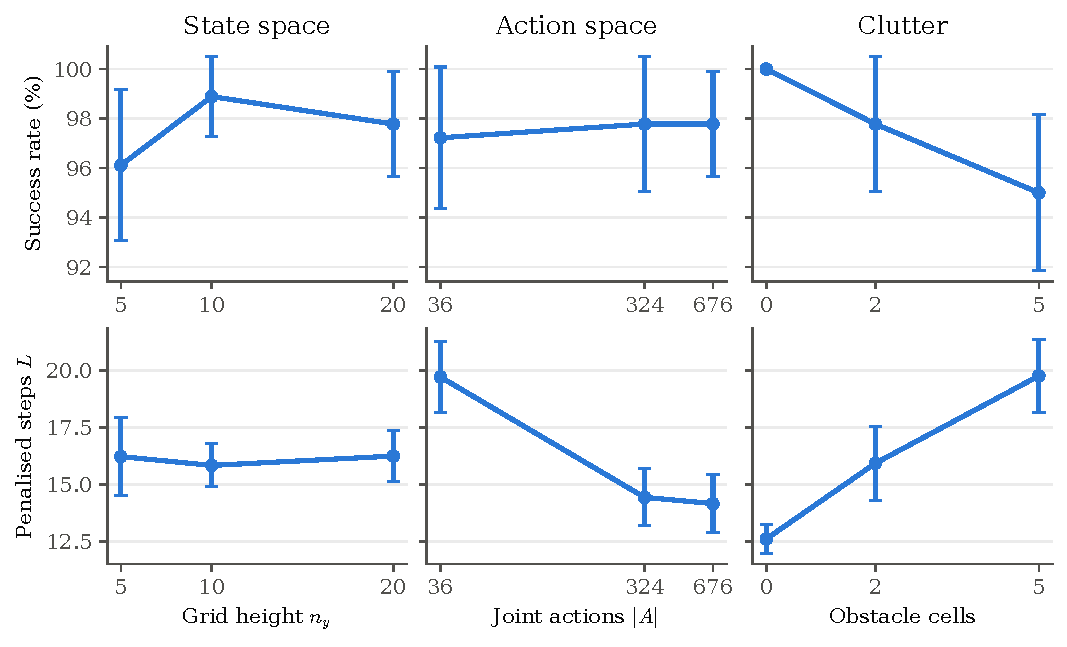
\includegraphics[width=0.95\linewidth]{figures/complexity_effects.pdf}
\caption{Factorial marginal means; bars are 95\% intervals over 20 seed blocks.}
\end{figure}
\begin{table}[H]
\centering\small
\begin{tabular}{@{}lll@{}}
\toprule Factor (high minus low) & $\Delta L$ (95\% CI) & $\Delta$success (pp; 95\% CI) \\
\midrule
\FactorEffectRows
\bottomrule
\end{tabular}
\end{table}

\textbf{Clutter causes the largest degradation within these tested levels.}
Adding five obstacles raises $L$ by $\val{EffCL}$ steps $\val{EffCLci}$ and
changes success by $\val{EffCP}$ percentage points $\val{EffCPci}$.
The solver succeeds in $\val{FactSuccess}\%$ of S1 episodes; all
$\val{FactCollisions}$ failures are collisions and none reaches the horizon.

\textbf{State-space padding has little observed effect.}
For $n_y=10$ versus 20, $\val{SameSTen}$ of $\val{SameSTotal}$ paired
episodes are identical. The extra off-route cells do not affect these runs;
this tests padding, not the effect of longer routes or additional drones.
Mean map setup grows from $\val{SetupS5}$ to $\val{SetupS20}$\,ms
($n_y=5$ versus 20), outside per-decision planning.

\textbf{Richer commands shorten routes.}
Changing 6 to 26 directions gives $\Delta L=\val{EffAL}$ $\val{EffALci}$;
the success difference is not statistically resolved.
The action--clutter interaction is $\val{IntAC}$ $\val{IntACci}$ steps,
consistent with diagonal/vertical moves easing obstacle
avoidance. Neither state-related interaction is resolved
($S\times C$: $\val{IntSCci}$; $S\times A$: $\val{IntSAci}$).

\subsubsection*{S2: geometry, noise and action branching}
At $n_y=10$, the clutter effect averaged over the two command sets is
$\val{ClutterNoisy}$ steps $\val{ClutterNoisyci}$ at $\alpha=0.25$,
versus $\val{ClutterQuiet}$ $\val{ClutterQuietci}$ at $\alpha=0.01$,
where all episodes succeed. Thus geometry still adds detour cost, while
noise substantially increases the observed clutter penalty.
The supplied transition law raises slip probability near obstacles;
its no-obstacle distance-transform convention is noted in
Appendix~\ref{app:guidance}.

Duplicating command labels up to $|A|=10{,}816$ changes $L$ by only
$\val{Branch}$ $\val{Branchci}$ and leaves the admitted root-action count
near 23. This separates pure label branching from the extra control
authority in S1. Detailed controls, including the visit share of the
\emph{executed} action, appear in Appendix~\ref{app:controls}.

\subsubsection*{S3: component effects as complexity increases}
\begin{figure}[!htbp]
\centering
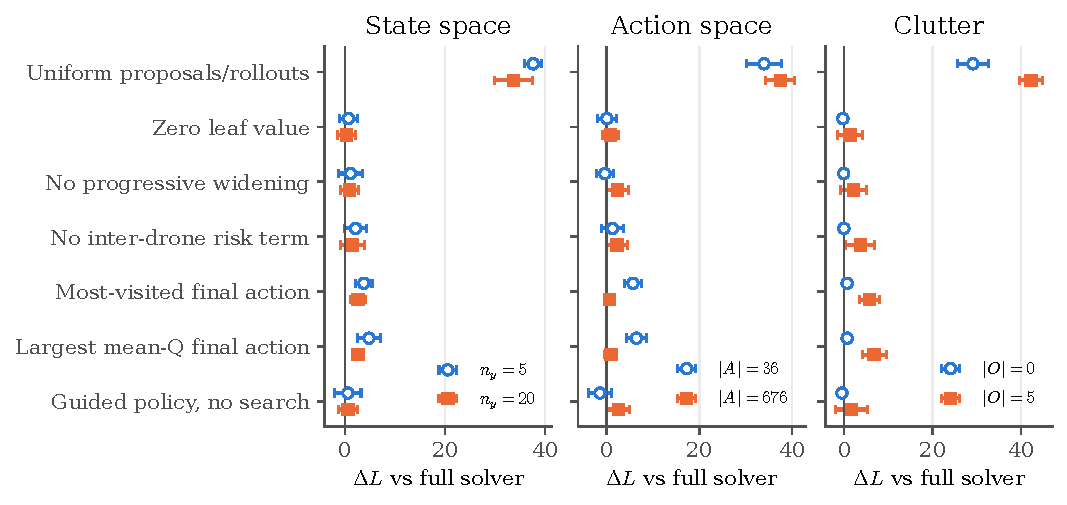
\includegraphics[width=\linewidth]{figures/component_effects.pdf}
\caption{Paired change in $L$ after removing a component at low/high factor
levels (open/filled markers); 95\% seed-block intervals.
Positive values favour the full solver.}
\end{figure}

\textbf{Guidance in expansion and rollout} has the largest measured effect.
Uniform proposals/rollouts raise $L$ by $\val{CompNoguidance}$
$\val{CompNoguidanceci}$ and change success by $\val{CompNoguidanceP}$\,pp.
The loss grows from $\val{CompNoguidanceClo}$ without obstacles to
$\val{CompNoguidanceChi}$ with five; the clutter interaction excludes zero
($\val{CompNoguidanceCint}$), whereas its state/action interactions do not.
This ablation removes both route guidance and admissible-target filtering.

\textbf{Root choice} also matters: most-visited selection raises $L$ by
$\val{CompVisitschoice}$ $\val{CompVisitschoiceci}$, and executing the
largest-mean-$Q$ action raises it by $\val{CompMaxq}$ $\val{CompMaxqci}$.
Both increases are larger with clutter (interaction intervals
$\val{CompVisitschoiceCint}$ and $\val{CompMaxqCint}$) and smaller with richer
commands ($\val{CompVisitschoiceAint}$ and $\val{CompMaxqAint}$). These
comparisons support the chosen switching rule on these tasks; they do not
make its estimated margin a calibrated confidence bound.

\textbf{Widening and the leaf value} have no statistically resolved effects
across these corners ($\val{CompNowidening}$ $\val{CompNowideningci}$ and
$\val{CompNoleaf}$ $\val{CompNoleafci}$; full estimates in
Appendix~\ref{app:components}). Routes are roughly eleven steps, comparable
to the sampled tree depth plus eight-step rollout, which may limit the leaf
value's contribution. \textbf{The inter-drone risk term} does matter:
removing it raises $L$ by $\val{CompNorisk}$ $\val{CompNoriskci}$ and changes
success by $\val{CompNoriskP}$\,pp, mostly with clutter (interaction
$\val{CompNoriskCint}$).

\textbf{Search versus its base policy.}
Removing search changes $L$ by $\val{CompHeuristic}$ $\val{CompHeuristicci}$
overall, but its action interaction is resolved ($\val{CompHeuristicAint}$):
removing search raises $L$ with 26 commands ($\val{CompHeuristicAhi}$),
while the change with 6 commands is unresolved ($\val{CompHeuristicAlo}$).
In the regression and generated suites, search rescues
$\val{BaseMultiRescued}$ multi-drone episodes and loses $\val{BaseMultiLost}$
and removing it changes $L$ by $\val{BaseMultiDL}$
$\val{BaseMultiDLci}$ (Appendix~\ref{app:regression}). With value guidance,
search has no consistent completion benefit across the evaluated suites;
the measured performance is largely explained by the guided base policy.


\subsubsection*{S4: search budget}
\begin{figure}[H]
\centering
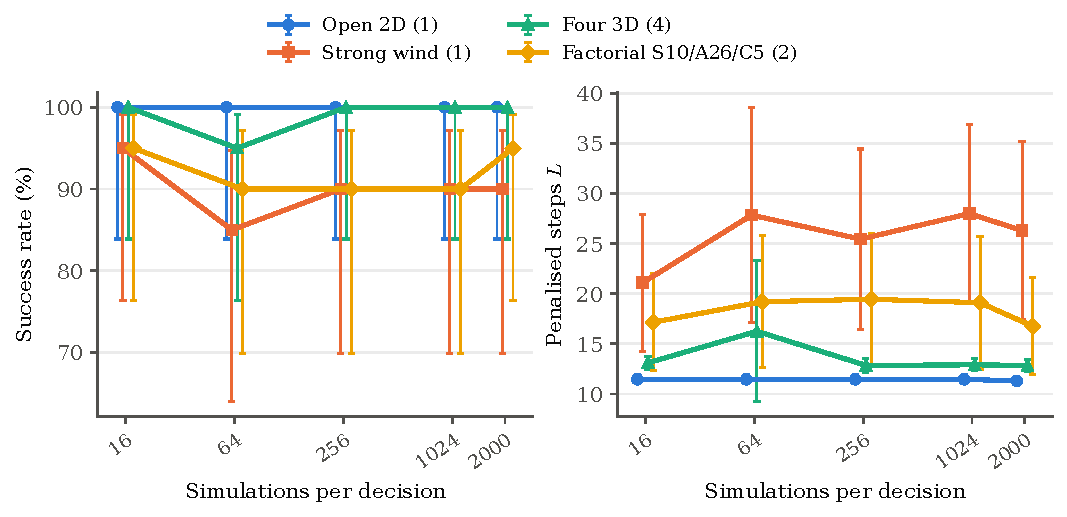
\includegraphics[width=0.95\linewidth]{figures/budget_curve.pdf}
\caption{Success and $L$ versus simulations per decision; 20 runs per point,
with Wilson and $t$ 95\% intervals. Drone counts are in parentheses.}
\end{figure}
There is no consistent improvement from 16 to 2,000 simulations across
these four tasks. In the four-drone case, success is
$\val{BudgetDemoFour3D16}$ and $\val{BudgetDemoFour3D2000}$ respectively,
while mean new-node depth grows from $\val{BudgetDemoFour3D16Depth}$ to
$\val{BudgetDemoFour3D2000Depth}$ and the fraction keeping the base action
falls from $\val{BudgetDemoFour3D16Kept}$ to $\val{BudgetDemoFour3D2000Kept}$.
Search therefore changes decisions without a demonstrated completion
benefit here. Overlapping intervals do not establish budget equivalence.

\subsubsection*{S5: generated layouts}
Across the crossed drone-count/noise set, $\val{RandOverall}$ episodes
succeed. At $\alpha\le0.25$, $\val{RandLowNoise}$ runs succeed,
including $\val{RandNFourLow}$ with four drones; four drones at $\alpha=2$
succeed in $\val{RandNFourHigh}$. This indicates sensitivity to noise in
the tested layouts, while increasing $N$ jointly enlarges state and action
spaces. Mean new-node depth is $\val{DepthN1}$ for one drone and
$\val{DepthN4}$ for four, consistent with less successor reuse when joint
outcomes multiply. Each $(N,\alpha)$ pair has only one layout, so the
per-layout results in Appendix~\ref{app:layouts} do not isolate layout effects.
For the four-drone layout at $\alpha=2$, joint value iteration was not attempted
($140^4\approx4\times10^8$ joint positions per step). Each drone alone could
achieve at least $\val{CeilFourSingle}\%$ success when other drones are removed.
Executing those policies together gives $\val{CeilFourUncoord}\%$ success
(1,000 diagnostic runs; Wilson 95\% interval $\val{CeilFourUncoordCI}$),
compared with $\val{RandNFourHigh}$ for the solver. The different sample sizes
and unpaired comparison do not establish a solver advantage or isolate the
cause of failure. They motivate further coordination tests
(\texttt{results/ceilings.json}).

\subsubsection*{Conclusions and limitations}
Within the factorial's tested levels, clutter causes the largest
degradation; extra control directions help, while off-route state padding
has little observed effect. Guided expansion/rollout and the root decision
rule contribute most, particularly in clutter. Additional search has no
demonstrated completion benefit over the guided base policy on these tasks.

The ranking is specific to two drones, $\alpha=0.25$ and the chosen layouts.
The $t$ intervals for bimodal $L$ are approximate, and generated-layout
replication is limited. Fixed-simulation experiments do not reproduce a
binding demo deadline on every machine. Static guidance does not model
detours around frozen drones beyond the leaf disconnection check; observed
collisions have not been proved unavoidable. The leaf estimate charges no
collision risk, so search can postpone an unavoidable risky passage beyond
its horizon: in the wall-gap case (Figure~\ref{fig:risk-maps}, bottom
right) successful runs averaged
$\val{SuppGapSteps}$ steps for an $\val{SuppGapRoute}$-step route. A
risk-charged leaf shortened those runs in a small probe
($\val{ProbeBaseGapSteps}$ to $\val{ProbeRiskGapSteps}$ steps) without raising
success ($\val{ProbeRisk}$ versus $\val{ProbeBase}$ over eight tasks), so it was
not adopted.
Stronger coordination tasks and outcome widening or open-loop
trees would be useful follow-up tests.

\par
\endgroup
